% ============================================================
% Question Bank: ch09-02 Theoretical Probability
% Topic Title: Theoretical Probability
% CCSS: 7.SP.C.6
% Questions: 30 (18 MC + 7 SA + 5 Graphical)
% ============================================================

% --- Multiple Choice Questions (18) ---

\begin{practiceQuestion}{9-2-q01}{mc}
\begin{questionText}
What is the theoretical probability of rolling a $3$ on a standard number cube?
\end{questionText}
\choiceA{$\frac{1}{3}$}
\choiceB{$\frac{1}{6}$}
\choiceC{$\frac{3}{6}$}
\choiceD{$\frac{1}{2}$}
\correctAnswer{B}
\explanation{There is $1$ favorable outcome ($3$) out of $6$ equally likely outcomes. $P = \frac{1}{6}$.}
\end{practiceQuestion}

\begin{practiceQuestion}{9-2-q02}{mc}
\begin{questionText}
A bag contains $8$ red marbles and $12$ blue marbles. What is the theoretical probability of drawing a red marble?
\end{questionText}
\choiceA{$\frac{8}{12}$}
\choiceB{$\frac{12}{20}$}
\choiceC{$\frac{2}{5}$}
\choiceD{$\frac{1}{8}$}
\correctAnswer{C}
\explanation{$P = \frac{8}{20} = \frac{2}{5}$.}
\end{practiceQuestion}

\begin{practiceQuestion}{9-2-q03}{mc}
\begin{questionText}
What is the probability of drawing a heart from a standard deck of $52$ cards?
\end{questionText}
\choiceA{$\frac{1}{13}$}
\choiceB{$\frac{1}{52}$}
\choiceC{$\frac{1}{2}$}
\choiceD{$\frac{1}{4}$}
\correctAnswer{D}
\explanation{There are $13$ hearts in a deck of $52$ cards. $P = \frac{13}{52} = \frac{1}{4}$.}
\end{practiceQuestion}

\begin{practiceQuestion}{9-2-q04}{mc}
\begin{questionText}
A standard number cube is rolled. What is the probability of rolling an even number?
\end{questionText}
\choiceA{$\frac{1}{6}$}
\choiceB{$\frac{1}{3}$}
\choiceC{$\frac{1}{2}$}
\choiceD{$\frac{2}{3}$}
\correctAnswer{C}
\explanation{Even numbers are $2, 4, 6$ — that is $3$ out of $6$. $P = \frac{3}{6} = \frac{1}{2}$.}
\end{practiceQuestion}

\begin{practiceQuestion}{9-2-q05}{mc}
\begin{questionText}
A spinner has $10$ equal sections numbered $1$ through $10$. What is the probability of landing on a number greater than $7$?
\end{questionText}
\choiceA{$\frac{7}{10}$}
\choiceB{$\frac{3}{10}$}
\choiceC{$\frac{3}{7}$}
\choiceD{$\frac{1}{10}$}
\correctAnswer{B}
\explanation{Numbers greater than $7$: $8, 9, 10$ — that is $3$ out of $10$. $P = \frac{3}{10}$.}
\end{practiceQuestion}

\begin{practiceQuestion}{9-2-q06}{mc}
\begin{questionText}
A bag contains $5$ green, $3$ yellow, and $2$ purple marbles. What is the probability of drawing a marble that is NOT purple?
\end{questionText}
\choiceA{$\frac{2}{10}$}
\choiceB{$\frac{3}{10}$}
\choiceC{$\frac{4}{5}$}
\choiceD{$\frac{1}{2}$}
\correctAnswer{C}
\explanation{Not purple: $5 + 3 = 8$ out of $10$ total. $P = \frac{8}{10} = \frac{4}{5}$.}
\end{practiceQuestion}

\begin{practiceQuestion}{9-2-q07}{mc}
\begin{questionText}
What is the probability of drawing a face card (Jack, Queen, or King) from a standard deck of $52$ cards?
\end{questionText}
\choiceA{$\frac{3}{52}$}
\choiceB{$\frac{3}{13}$}
\choiceC{$\frac{1}{4}$}
\choiceD{$\frac{4}{13}$}
\correctAnswer{B}
\explanation{There are $3$ face cards per suit $\times$ $4$ suits $= 12$ face cards. $P = \frac{12}{52} = \frac{3}{13}$.}
\end{practiceQuestion}

\begin{practiceQuestion}{9-2-q08}{mc}
\begin{questionText}
A jar contains $6$ red, $4$ blue, and $10$ white gumballs. What is the probability of drawing a blue gumball?
\end{questionText}
\choiceA{$\frac{1}{4}$}
\choiceB{$\frac{2}{5}$}
\choiceC{$\frac{1}{5}$}
\choiceD{$\frac{4}{10}$}
\correctAnswer{C}
\explanation{Total gumballs: $6 + 4 + 10 = 20$. $P = \frac{4}{20} = \frac{1}{5}$.}
\end{practiceQuestion}

\begin{practiceQuestion}{9-2-q09}{mc}
\begin{questionText}
The letters of the word STATISTICS are placed in a bag. What is the probability of drawing the letter S?
\end{questionText}
\choiceA{$\frac{1}{10}$}
\choiceB{$\frac{2}{10}$}
\choiceC{$\frac{3}{10}$}
\choiceD{$\frac{4}{10}$}
\correctAnswer{C}
\explanation{STATISTICS has $10$ letters: S, T, A, T, I, S, T, I, C, S. The letter S appears $3$ times. $P = \frac{3}{10}$.}
\end{practiceQuestion}

\begin{practiceQuestion}{9-2-q10}{mc}
\begin{questionText}
A number cube is rolled. What is the probability of rolling a number that is a multiple of $3$?
\end{questionText}
\choiceA{$\frac{1}{6}$}
\choiceB{$\frac{1}{3}$}
\choiceC{$\frac{1}{2}$}
\choiceD{$\frac{2}{3}$}
\correctAnswer{B}
\explanation{Multiples of $3$ on a die: $3$ and $6$ — that is $2$ out of $6$. $P = \frac{2}{6} = \frac{1}{3}$.}
\end{practiceQuestion}

\begin{practiceQuestion}{9-2-q11}{mc}
\begin{questionText}
A bag has $3$ red, $3$ blue, and $3$ green marbles. Carlos says the probability of drawing a red marble is $\frac{1}{3}$. Is he correct?
\end{questionText}
\choiceA{No, the probability is $\frac{3}{6}$}
\choiceB{No, the probability is $\frac{1}{9}$}
\choiceC{Yes, because $3$ out of $9$ is $\frac{1}{3}$}
\choiceD{Yes, because there are $3$ colors}
\correctAnswer{C}
\explanation{$P = \frac{3}{9} = \frac{1}{3}$. Carlos is correct.}
\end{practiceQuestion}

\begin{practiceQuestion}{9-2-q12}{mc}
\begin{questionText}
What is the probability of randomly selecting a vowel from the letters of the word PROBABILITY?
\end{questionText}
\choiceA{$\frac{3}{11}$}
\choiceB{$\frac{4}{11}$}
\choiceC{$\frac{5}{11}$}
\choiceD{$\frac{2}{11}$}
\correctAnswer{B}
\explanation{PROBABILITY has $11$ letters: P, R, O, B, A, B, I, L, I, T, Y. Vowels: O, A, I, I — that is $4$. $P = \frac{4}{11}$.}
\end{practiceQuestion}

\begin{practiceQuestion}{9-2-q13}{mc}
\begin{questionText}
A standard deck of cards has $52$ cards. What is the probability of drawing a card that is a $2$ or a $3$?
\end{questionText}
\choiceA{$\frac{2}{52}$}
\choiceB{$\frac{4}{52}$}
\choiceC{$\frac{2}{13}$}
\choiceD{$\frac{1}{13}$}
\correctAnswer{C}
\explanation{There are $4$ twos and $4$ threes $= 8$ cards. $P = \frac{8}{52} = \frac{2}{13}$.}
\end{practiceQuestion}

\begin{practiceQuestion}{9-2-q14}{mc}
\begin{questionText}
A bag contains $15$ marbles: $5$ are striped, $10$ are solid. What is the probability that a randomly chosen marble is striped?
\end{questionText}
\choiceA{$\frac{1}{5}$}
\choiceB{$\frac{1}{3}$}
\choiceC{$\frac{2}{3}$}
\choiceD{$\frac{1}{15}$}
\correctAnswer{B}
\explanation{$P = \frac{5}{15} = \frac{1}{3}$.}
\end{practiceQuestion}

\begin{practiceQuestion}{9-2-q15}{mc}
\begin{questionText}
Two number cubes are rolled. How many total outcomes are in the sample space?
\end{questionText}
\choiceA{$6$}
\choiceB{$12$}
\choiceC{$36$}
\choiceD{$24$}
\correctAnswer{C}
\explanation{Each cube has $6$ outcomes. $6 \times 6 = 36$ total outcomes.}
\end{practiceQuestion}

\begin{practiceQuestion}{9-2-q16}{mc}
\begin{questionText}
A spinner has $5$ equal sections labeled $1$ through $5$. What is the probability of spinning a prime number?
\end{questionText}
\choiceA{$\frac{1}{5}$}
\choiceB{$\frac{2}{5}$}
\choiceC{$\frac{3}{5}$}
\choiceD{$\frac{4}{5}$}
\correctAnswer{C}
\explanation{Prime numbers from $1$ to $5$: $2, 3, 5$ — that is $3$ out of $5$. $P = \frac{3}{5}$.}
\end{practiceQuestion}

\begin{practiceQuestion}{9-2-q17}{mc}
\begin{questionText}
A coin is flipped and a die is rolled. What is the probability of getting heads and a $4$?
\end{questionText}
\choiceA{$\frac{1}{6}$}
\choiceB{$\frac{1}{12}$}
\choiceC{$\frac{1}{8}$}
\choiceD{$\frac{1}{2}$}
\correctAnswer{B}
\explanation{$P(\text{heads}) = \frac{1}{2}$ and $P(4) = \frac{1}{6}$. $P = \frac{1}{2} \times \frac{1}{6} = \frac{1}{12}$.}
\end{practiceQuestion}

\begin{practiceQuestion}{9-2-q18}{mc}
\begin{questionText}
A jar has $4$ red, $6$ blue, and $2$ yellow candies. If you pick one candy at random, which color are you MOST likely to pick?
\end{questionText}
\choiceA{Red}
\choiceB{Blue}
\choiceC{Yellow}
\choiceD{All are equally likely}
\correctAnswer{B}
\explanation{Blue has the most candies ($6$ out of $12$), so it is the most likely to be picked.}
\end{practiceQuestion}

% --- Short Answer Questions (7) ---

\begin{practiceQuestion}{9-2-q19}{sa}
\begin{questionText}
A bag contains $9$ red and $6$ green marbles. What is the theoretical probability of drawing a green marble? Write your answer as a simplified fraction.
\end{questionText}
\correctAnswer{$\frac{2}{5}$}
\explanation{$P = \frac{6}{15} = \frac{2}{5}$.}
\end{practiceQuestion}

\begin{practiceQuestion}{9-2-q20}{sa}
\begin{questionText}
A standard number cube is rolled. What is the probability of rolling a $1$ or a $5$? Write your answer as a fraction in simplest form.
\end{questionText}
\correctAnswer{$\frac{1}{3}$}
\explanation{Favorable outcomes: $1$ and $5$ — that is $2$ out of $6$. $P = \frac{2}{6} = \frac{1}{3}$.}
\end{practiceQuestion}

\begin{practiceQuestion}{9-2-q21}{sa}
\begin{questionText}
There are $20$ students in a class. $8$ students have brown hair. What is the probability that a randomly selected student has brown hair? Write your answer as a decimal.
\end{questionText}
\correctAnswer{$0.4$}
\explanation{$P = \frac{8}{20} = 0.4$.}
\end{practiceQuestion}

\begin{practiceQuestion}{9-2-q22}{sa}
\begin{questionText}
A bag has $10$ tiles numbered $1$ through $10$. What is the probability of drawing an odd number? Write your answer as a fraction.
\end{questionText}
\correctAnswer{$\frac{1}{2}$}
\explanation{Odd numbers: $1, 3, 5, 7, 9$ — that is $5$ out of $10$. $P = \frac{5}{10} = \frac{1}{2}$.}
\end{practiceQuestion}

\begin{practiceQuestion}{9-2-q23}{sa}
\begin{questionText}
What is the probability of drawing a King from a standard deck of $52$ cards? Write your answer as a fraction in simplest form.
\end{questionText}
\correctAnswer{$\frac{1}{13}$}
\explanation{There are $4$ Kings. $P = \frac{4}{52} = \frac{1}{13}$.}
\end{practiceQuestion}

\begin{practiceQuestion}{9-2-q24}{sa}
\begin{questionText}
A spinner has $6$ equal sections colored red, red, blue, blue, blue, and green. What is the probability of NOT landing on blue? Write your answer as a fraction in simplest form.
\end{questionText}
\correctAnswer{$\frac{1}{2}$}
\explanation{Blue occupies $3$ sections. Not blue $= 6 - 3 = 3$ sections. $P = \frac{3}{6} = \frac{1}{2}$.}
\end{practiceQuestion}

\begin{practiceQuestion}{9-2-q25}{sa}
\begin{questionText}
A coin is flipped $3$ times. How many outcomes are in the sample space?
\end{questionText}
\correctAnswer{$8$}
\explanation{$2 \times 2 \times 2 = 8$ possible outcomes.}
\end{practiceQuestion}

% --- Graphical Questions (3 GMC + 2 GSA) ---

\begin{practiceQuestion}{9-2-q26}{gmc}
\begin{questionText}
A spinner is divided into sections as shown below. What is the theoretical probability of landing on section $B$?

\begin{center}
\begin{tikzpicture}[scale=1.2]
  \fill[funRed!50] (0,0) -- (0:1.5) arc (0:90:1.5) -- cycle;
  \fill[funBlue!50] (0,0) -- (90:1.5) arc (90:180:1.5) -- cycle;
  \fill[funGreen!50] (0,0) -- (180:1.5) arc (180:270:1.5) -- cycle;
  \fill[funOrange!50] (0,0) -- (270:1.5) arc (270:360:1.5) -- cycle;
  \draw[thick] (0,0) circle (1.5);
  \draw[thick] (0,0) -- (0:1.5);
  \draw[thick] (0,0) -- (90:1.5);
  \draw[thick] (0,0) -- (180:1.5);
  \draw[thick] (0,0) -- (270:1.5);
  \node[font=\bfseries] at (45:0.8) {A};
  \node[font=\bfseries] at (135:0.8) {B};
  \node[font=\bfseries] at (225:0.8) {C};
  \node[font=\bfseries] at (315:0.8) {D};
\end{tikzpicture}
\end{center}
\end{questionText}
\choiceA{$\frac{1}{2}$}
\choiceB{$\frac{1}{3}$}
\choiceC{$\frac{1}{4}$}
\choiceD{$\frac{1}{6}$}
\correctAnswer{C}
\explanation{The spinner has $4$ equal sections, so each section has probability $\frac{1}{4}$.}
\end{practiceQuestion}

\begin{practiceQuestion}{9-2-q27}{gmc}
\begin{questionText}
Look at the contents of the bag below. What is the probability of drawing a star-shaped token?

\begin{center}
\begin{tikzpicture}[scale=0.7]
  \draw[thick,rounded corners=10pt] (-3,-2) rectangle (3,2);
  % Circles (4)
  \fill[funRed!60] (-2,0.8) circle (0.3);
  \fill[funRed!60] (-0.5,0.8) circle (0.3);
  \fill[funRed!60] (1,0.8) circle (0.3);
  \fill[funRed!60] (2.2,0.8) circle (0.3);
  % Stars (3)
  \foreach \cx in {-1.5, 0.3, 1.8} {
    \fill[funBlue!60] (\cx,-0.7) -- ++(0.15,0.35) -- ++(0.35,0) -- ++(-0.25,0.25) -- ++(0.1,0.35) -- ++(-0.35,-0.2) -- ++(-0.35,0.2) -- ++(0.1,-0.35) -- ++(-0.25,-0.25) -- ++(0.35,0) -- cycle;
  }
  \node[below,font=\small] at (-2,0.35) {circle};
  \node[below,font=\small] at (0.3,-1.2) {star};
\end{tikzpicture}
\end{center}
\end{questionText}
\choiceA{$\frac{4}{7}$}
\choiceB{$\frac{3}{7}$}
\choiceC{$\frac{3}{4}$}
\choiceD{$\frac{1}{3}$}
\correctAnswer{B}
\explanation{There are $4$ circles and $3$ stars, for $7$ tokens total. $P(\text{star}) = \frac{3}{7}$.}
\end{practiceQuestion}

\begin{practiceQuestion}{9-2-q28}{gmc}
\begin{questionText}
The table below shows the number of each color of candy in a bag. If you randomly pick one candy, what is the probability of picking a green candy?

\begin{center}
\begin{tabular}{|c|c|}
\hline
\textbf{Color} & \textbf{Number} \\
\hline
Red & $6$ \\
\hline
Green & $9$ \\
\hline
Yellow & $5$ \\
\hline
Orange & $5$ \\
\hline
\end{tabular}
\end{center}
\end{questionText}
\choiceA{$\frac{9}{25}$}
\choiceB{$\frac{9}{20}$}
\choiceC{$\frac{1}{4}$}
\choiceD{$\frac{9}{15}$}
\correctAnswer{A}
\explanation{Total candies: $6 + 9 + 5 + 5 = 25$. $P(\text{green}) = \frac{9}{25}$.}
\end{practiceQuestion}

\begin{practiceQuestion}{9-2-q29}{gsa}
\begin{questionText}
A number line shows equally spaced points. Each point represents a possible outcome when a spinner is spun. What is the probability of the spinner landing on a point between $3$ and $5$ (not including $3$ and $5$)?

\begin{center}
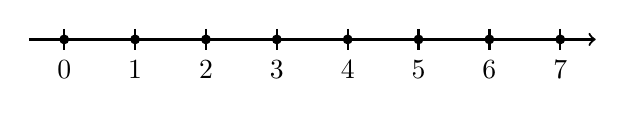
\begin{tikzpicture}[scale=0.9]
  \draw[thick,->] (-0.5,0) -- (7.5,0);
  \foreach \x in {0,...,7} {
    \draw[thick] (\x,0.15) -- (\x,-0.15) node[below] {$\x$};
    \fill (\x,0) circle (0.07);
  }
\end{tikzpicture}
\end{center}
\end{questionText}
\correctAnswer{$\frac{1}{8}$}
\explanation{The points are $0, 1, 2, 3, 4, 5, 6, 7$ — that is $8$ equally likely outcomes. The only point strictly between $3$ and $5$ is $4$. $P = \frac{1}{8}$.}
\end{practiceQuestion}

\begin{practiceQuestion}{9-2-q30}{gsa}
\begin{questionText}
The bar graph shows how many marbles of each color are in a bag. What is the probability of drawing a marble that is either red or yellow? Write your answer as a fraction in simplest form.

\begin{center}
\begin{tikzpicture}[scale=0.55]
  \draw[thick,->] (0,0) -- (0,9) node[above,font=\small] {Count};
  \draw[thick,->] (0,0) -- (9,0);
  \foreach \y in {1,...,8} {
    \draw[gray!40] (0,\y) -- (8.5,\y);
    \node[left,font=\small] at (0,\y) {\y};
  }
  \fill[funRed!70] (0.5,0) rectangle (1.5,4);
  \fill[funBlue!70] (2.5,0) rectangle (3.5,6);
  \fill[funYellow!70] (4.5,0) rectangle (5.5,2);
  \fill[funGreen!70] (6.5,0) rectangle (7.5,8);
  \node[below,font=\small] at (1,0) {Red};
  \node[below,font=\small] at (3,0) {Blue};
  \node[below,font=\small] at (5,0) {Yel.};
  \node[below,font=\small] at (7,0) {Grn.};
\end{tikzpicture}
\end{center}
\end{questionText}
\correctAnswer{$\frac{3}{10}$}
\explanation{Red $= 4$, Blue $= 6$, Yellow $= 2$, Green $= 8$. Total $= 20$. Red or Yellow $= 4 + 2 = 6$. $P = \frac{6}{20} = \frac{3}{10}$.}
\end{practiceQuestion}
